\section{Overview}

The cryptographic core of the Feedback-Coupled Cryptographic Observation (RCO) protocol defines the formal mechanisms by which telemetry data is transformed into a deterministic, immutable, and verifiable representation suitable for use in feedback-coupled computational systems. Unlike conventional cryptographic applications that operate on static data, the present framework operates on temporally evolving telemetry sequences that directly influence system dynamics. Consequently, the cryptographic core must enforce not only classical security properties such as collision resistance and unforgeability, but also structural invariants that guarantee deterministic behavior across heterogeneous computational environments.

Let $\mathcal{D}$ denote the space of telemetry data and $\{D_t\}_{t=0}^{T}$ a sequence of telemetry elements. The cryptographic core defines a transformation:

\begin{equation}
\mathcal{K}: \mathcal{D}^{T} \rightarrow \mathcal{L}^{T}
\end{equation}

where $\mathcal{L}$ denotes the lineage space. The transformation $\mathcal{K}$ must satisfy the following global invariant:

\begin{equation}
\forall D, \tilde{D} \in \mathcal{D}^{T}, \quad D \equiv \tilde{D} \implies \mathcal{K}(D) = \mathcal{K}(\tilde{D})
\end{equation}

ensuring that semantically equivalent telemetry sequences produce identical cryptographic representations.

This requirement imposes a stricter condition than standard cryptographic hashing, as it necessitates determinism at the level of input representation prior to hashing. The cryptographic core is therefore decomposed into three primary operators:

\begin{equation}
\mathcal{K} = \mathcal{C} \circ \mathcal{H} \circ \mathcal{S}
\end{equation}

where $\mathcal{S}$ is a canonical serialization operator, $\mathcal{H}$ is a cryptographic hashing operator, and $\mathcal{C}$ is a chaining operator that constructs lineage.

\section{Deterministic Serialization Layer}

The deterministic serialization layer constitutes the foundational component of the cryptographic core, as it ensures that all subsequent cryptographic operations operate on a uniquely defined binary representation. Without this property, the guarantees provided by cryptographic hashing and chaining are invalidated, as identical logical inputs may produce divergent outputs.

\subsection{Formal Definition of Serialization}

Let $\mathcal{D}$ denote the space of structured telemetry data, which may be represented as a finite set of key-value pairs:

\begin{equation}
D = \{(k_i, v_i)\}_{i=1}^{n}
\end{equation}

where $k_i \in \mathcal{K}$ and $v_i \in \mathcal{V}$. A serialization function is defined as:

\begin{equation}
\mathcal{S}: \mathcal{D} \rightarrow \{0,1\}^*
\end{equation}

mapping structured data into a binary sequence.

The serialization function is said to be canonical if it satisfies:

\begin{equation}
D_1 \equiv D_2 \implies \mathcal{S}(D_1) = \mathcal{S}(D_2)
\end{equation}

This property defines injective consistency with respect to semantic equivalence.

\subsection{Non-Determinism in Conventional Serialization}

In conventional systems, serialization functions fail to satisfy the canonical property. Consider two equivalent representations of a dictionary:

\begin{equation}
D_1 = \{(k_1, v_1), (k_2, v_2)\}, \quad D_2 = \{(k_2, v_2), (k_1, v_1)\}
\end{equation}

Then:

\begin{equation}
\mathcal{S}(D_1) \neq \mathcal{S}(D_2)
\end{equation}

in the absence of enforced ordering. This violation introduces ambiguity in downstream cryptographic operations.

Furthermore, for numerical values $x \in \mathbb{R}$, floating-point representations introduce additional non-determinism. Let $\mathcal{F}_i$ denote the floating-point encoding under architecture $i$. Then:

\begin{equation}
\mathcal{F}_i(x) \neq \mathcal{F}_j(x)
\end{equation}

for certain values of $x$, particularly when rounding behavior differs.

\subsection{Canonical Serialization Construction}

To eliminate these sources of non-determinism, the serialization function $\mathcal{S}$ is constructed as a composition:

\begin{equation}
\mathcal{S} = \mathcal{E}_{\text{struct}} \circ \Pi_k
\end{equation}

where $\Pi_k$ is a fixed-precision projection operator and $\mathcal{E}_{\text{struct}}$ is a structural encoding function.

The projection operator is defined as:

\begin{equation}
\Pi_k: \mathbb{R} \rightarrow \mathbb{Z}, \quad \Pi_k(x) = \lfloor x \cdot 10^k \rfloor
\end{equation}

and extended component-wise to structured data:

\begin{equation}
\Pi_k(D) = \{(k_i, \Pi_k(v_i))\}_{i=1}^{n}
\end{equation}

This transformation maps real-valued inputs into a discrete lattice, eliminating floating-point inconsistencies.

The structural encoding function $\mathcal{E}_{\text{struct}}$ enforces a total ordering over keys. Let $\prec$ denote a lexicographic ordering over $\mathcal{K}$. Then:

\begin{equation}
\mathcal{E}_{\text{struct}}(D) = \text{Encode}(\{(k_{\pi(i)}, v_{\pi(i)})\}_{i=1}^{n})
\end{equation}

where $\pi$ is a permutation such that:

\begin{equation}
k_{\pi(1)} \prec k_{\pi(2)} \prec \dots \prec k_{\pi(n)}
\end{equation}

This ensures that the ordering of elements is uniquely defined.

\subsection{Determinism Theorem}

\begin{theorem}[Canonical Determinism]
The serialization function $\mathcal{S} = \mathcal{E}_{\text{struct}} \circ \Pi_k$ is canonical, i.e.,

\[
D_1 \equiv D_2 \implies \mathcal{S}(D_1) = \mathcal{S}(D_2)
\]
\end{theorem}

\begin{proof}
Assume $D_1 \equiv D_2$. Then for each key $k$, the corresponding values satisfy $v_1 = v_2$. Applying $\Pi_k$ yields identical integer representations:

\[
\Pi_k(v_1) = \Pi_k(v_2)
\]

Since both datasets contain identical key-value pairs, sorting under lexicographic order produces identical sequences. Therefore, the structural encoding produces identical outputs:

\[
\mathcal{E}_{\text{struct}}(\Pi_k(D_1)) = \mathcal{E}_{\text{struct}}(\Pi_k(D_2))
\]

Thus:

\[
\mathcal{S}(D_1) = \mathcal{S}(D_2)
\]

which completes the proof.
\end{proof}

\subsection{Cross-Platform Consistency}

Let $\mathcal{S}_i$ denote the serialization function executed on platform $i$. The use of fixed-precision projection ensures:

\begin{equation}
\forall i,j, \quad \mathcal{S}_i(D) = \mathcal{S}_j(D)
\end{equation}

as $\Pi_k$ eliminates floating-point discrepancies and $\mathcal{E}_{\text{struct}}$ enforces deterministic ordering independent of platform.

\subsection{Stability Under Perturbation}

Consider a perturbation $\delta$ applied to a numerical value $x$ such that $| \delta | < 10^{-k}$. Then:

\begin{equation}
\Pi_k(x + \delta) = \Pi_k(x)
\end{equation}

provided that the perturbation does not cross a quantization boundary. This implies that the serialization function is robust to small perturbations within quantization limits, preventing minor numerical noise from affecting the encoded representation.

\subsection{Entropy Preservation}

Let $H(D)$ denote the entropy of the telemetry data. The projection operator $\Pi_k$ introduces quantization, reducing entropy:

\begin{equation}
H(\Pi_k(D)) \leq H(D)
\end{equation}

However, this reduction is controlled by the choice of $k$, allowing a trade-off between precision and determinism. The structural encoding preserves entropy with respect to ordering, as it introduces no additional ambiguity.

\subsection{Implications for Cryptographic Processing}

The canonical serialization function ensures that all subsequent cryptographic operations operate on a stable and unique representation. In particular, for any hash function $\mathcal{H}$:

\begin{equation}
\mathcal{H}(\mathcal{S}(D_1)) = \mathcal{H}(\mathcal{S}(D_2)) \iff D_1 \equiv D_2
\end{equation}

under the assumption that $\mathcal{H}$ is collision-resistant. This establishes the necessary precondition for reliable hashing and lineage construction.

In summary, the deterministic serialization layer eliminates all sources of representation-induced ambiguity by enforcing canonical ordering and fixed-precision normalization. This layer provides the foundation upon which the remaining components of the cryptographic core are constructed, ensuring that the integrity guarantees of the system are preserved across heterogeneous environments and repeated executions.

\section{Cryptographic Hashing Layer}

The cryptographic hashing layer transforms the canonical binary representation of telemetry data into a fixed-length digest that serves as the fundamental unit of integrity within the RCO protocol. While the deterministic serialization layer ensures that semantically equivalent inputs produce identical binary encodings, the hashing layer ensures that any deviation in this encoding is reflected in a corresponding change in the hash output with overwhelming probability. The hashing function thus acts as a sensitivity amplifier, converting even minimal differences in input into statistically independent outputs.

Let $\mathcal{H}: \{0,1\}^* \rightarrow \{0,1\}^k$ denote a cryptographic hash function mapping arbitrary-length inputs to fixed-length outputs of size $k$. The choice of $\mathcal{H}$ must satisfy standard cryptographic security properties, which are formally defined below.

\subsection{Preimage Resistance}

The hash function $\mathcal{H}$ is said to be preimage-resistant if, given a hash value $y \in \{0,1\}^k$, it is computationally infeasible to find an input $x \in \{0,1\}^*$ such that:

\begin{equation}
\mathcal{H}(x) = y
\end{equation}

Formally, for any probabilistic polynomial-time adversary $\mathcal{A}$:

\begin{equation}
\Pr[\mathcal{A}(y) = x \text{ such that } \mathcal{H}(x) = y] \leq \epsilon
\end{equation}

where $\epsilon$ is negligible in $k$. This property ensures that given a lineage hash $L_t$, an adversary cannot reconstruct the underlying telemetry data.

\subsection{Second-Preimage Resistance}

The hash function is second-preimage resistant if, given an input $x$, it is computationally infeasible to find a distinct input $x' \neq x$ such that:

\begin{equation}
\mathcal{H}(x') = \mathcal{H}(x)
\end{equation}

Formally:

\begin{equation}
\Pr[\mathcal{A}(x) = x' \neq x \text{ such that } \mathcal{H}(x') = \mathcal{H}(x)] \leq \epsilon
\end{equation}

This property is essential for ensuring that an adversary cannot replace a telemetry entry with a different one that yields the same hash.

\subsection{Collision Resistance}

The hash function is collision-resistant if it is computationally infeasible to find any pair of distinct inputs $(x, x')$ such that:

\begin{equation}
\mathcal{H}(x) = \mathcal{H}(x')
\end{equation}

Formally:

\begin{equation}
\Pr[\mathcal{A}() = (x, x') \text{ with } x \neq x' \text{ and } \mathcal{H}(x) = \mathcal{H}(x')] \leq \epsilon
\end{equation}

Collision resistance ensures that the lineage structure uniquely represents the telemetry sequence.

\subsection{Content Hash Definition}

Given a telemetry element $D_t$, its canonical encoding is $\mathcal{S}(D_t)$. The content hash is defined as:

\begin{equation}
H_t = \mathcal{H}(\mathcal{S}(D_t))
\end{equation}

This hash serves as a compact representation of the telemetry element.

\subsection{Avalanche Property and Sensitivity Amplification}

A desirable property of $\mathcal{H}$ is the avalanche effect, whereby a single-bit change in the input results in a statistically independent output. Let $x$ and $x'$ differ by a single bit. Then:

\begin{equation}
\Pr[\mathcal{H}(x)_i \neq \mathcal{H}(x')_i] \approx \frac{1}{2}
\end{equation}

for each output bit $i$. This ensures that even minimal perturbations in the serialized telemetry result in large changes in the hash output.

From the perspective of Causative Telemetry Distortion, this property ensures that any non-zero perturbation $\delta_t$ in the serialized representation leads to:

\begin{equation}
H_t \neq H_t'
\end{equation}

with overwhelming probability, thereby making inconsistencies detectable.

\subsection{Adversarial Model}

Consider an adversary $\mathcal{A}$ attempting to manipulate telemetry data. The adversary may attempt to construct an alternative telemetry element $D_t'$ such that:

\begin{equation}
\mathcal{H}(\mathcal{S}(D_t')) = \mathcal{H}(\mathcal{S}(D_t))
\end{equation}

This constitutes a second-preimage attack. Under the assumption that $\mathcal{H}$ is second-preimage resistant, the probability of success is bounded by:

\begin{equation}
\Pr[\text{Success}] \leq 2^{-k}
\end{equation}

which is negligible for sufficiently large $k$.

Alternatively, the adversary may attempt to find any two distinct telemetry elements $D_t$ and $D_t'$ such that:

\begin{equation}
\mathcal{H}(\mathcal{S}(D_t)) = \mathcal{H}(\mathcal{S}(D_t'))
\end{equation}

This constitutes a collision attack. The expected complexity of such an attack is:

\begin{equation}
O(2^{k/2})
\end{equation}

due to the birthday bound. For $k = 256$, this corresponds to approximately $2^{128}$ operations, which is computationally infeasible.

\subsection{Hash Function as a Random Oracle Approximation}

In the security analysis of the RCO protocol, the hash function $\mathcal{H}$ may be modeled as a random oracle. That is, $\mathcal{H}$ is treated as a function that maps inputs to uniformly random outputs, subject to consistency constraints. Under this model, for any distinct inputs $x \neq x'$:

\begin{equation}
\Pr[\mathcal{H}(x) = \mathcal{H}(x')] = 2^{-k}
\end{equation}

This abstraction simplifies the analysis of lineage integrity and proof unforgeability.

\subsection{Entropy Compression and Information Preservation}

The hash function compresses input data of arbitrary length into a fixed-length output. Let $H(\cdot)$ denote entropy. Then:

\begin{equation}
H(H_t) \leq k
\end{equation}

while the input entropy $H(\mathcal{S}(D_t))$ may be significantly larger. Despite this compression, collision resistance ensures that distinct inputs remain distinguishable with high probability.

\subsection{Compositional Integrity with Serialization}

The combination of canonical serialization and cryptographic hashing yields a composite function:

\begin{equation}
\mathcal{H} \circ \mathcal{S}: \mathcal{D} \rightarrow \{0,1\}^k
\end{equation}

which satisfies:

\begin{equation}
D_1 \equiv D_2 \implies \mathcal{H}(\mathcal{S}(D_1)) = \mathcal{H}(\mathcal{S}(D_2))
\end{equation}

and:

\begin{equation}
D_1 \not\equiv D_2 \implies \Pr[\mathcal{H}(\mathcal{S}(D_1)) = \mathcal{H}(\mathcal{S}(D_2))] \leq 2^{-k}
\end{equation}

This establishes that the composite function is both deterministic and collision-resistant with respect to semantic equivalence.

\subsection{Robustness Against Structural Attacks}

An adversary may attempt to exploit structural properties of the serialization to produce collisions. However, the canonical nature of $\mathcal{S}$ ensures that the input space is well-defined and free of ambiguity. Combined with the cryptographic properties of $\mathcal{H}$, this prevents structural manipulation from yielding identical hash outputs.

\subsection{Implications for Lineage Construction}

The content hash $H_t$ serves as the input to the chaining operator. The security of the lineage structure depends critically on the properties of $\mathcal{H}$. In particular, the collision resistance of $\mathcal{H}$ ensures that the lineage uniquely represents the sequence of telemetry elements.

In summary, the cryptographic hashing layer provides a mechanism for transforming deterministic telemetry representations into fixed-length digests that preserve integrity and detect any deviation with overwhelming probability. By satisfying preimage resistance, second-preimage resistance, and collision resistance, the hash function ensures that the telemetry data cannot be manipulated without detection, forming a critical component of the RCO protocol.

\section{Merkle-Lineage Construction}

The Merkle-Lineage construction constitutes the temporal integrity backbone of the RCO protocol. While the hashing layer ensures that individual telemetry elements are uniquely represented, it does not by itself enforce any relationship between successive elements. The lineage construction introduces a recursive dependency structure over the sequence of telemetry data, ensuring that the integrity of the entire history is cryptographically bound to the current state.

Let $\{D_t\}_{t=0}^{T}$ denote a sequence of telemetry elements and $\{H_t\}_{t=0}^{T}$ their corresponding content hashes, where:

\begin{equation}
H_t = \mathcal{H}(\mathcal{S}(D_t))
\end{equation}

The lineage sequence $\{L_t\}_{t=0}^{T}$ is defined recursively as:

\begin{equation}
L_t = \mathcal{H}(H_t \concat L_{t-1})
\end{equation}

with an initial condition:

\begin{equation}
L_0 = \mathcal{H}(H_0 \concat \mathsf{IV})
\end{equation}

where $\mathsf{IV}$ is a fixed initialization vector or genesis constant.

\begin{figure}[htbp]
\centering
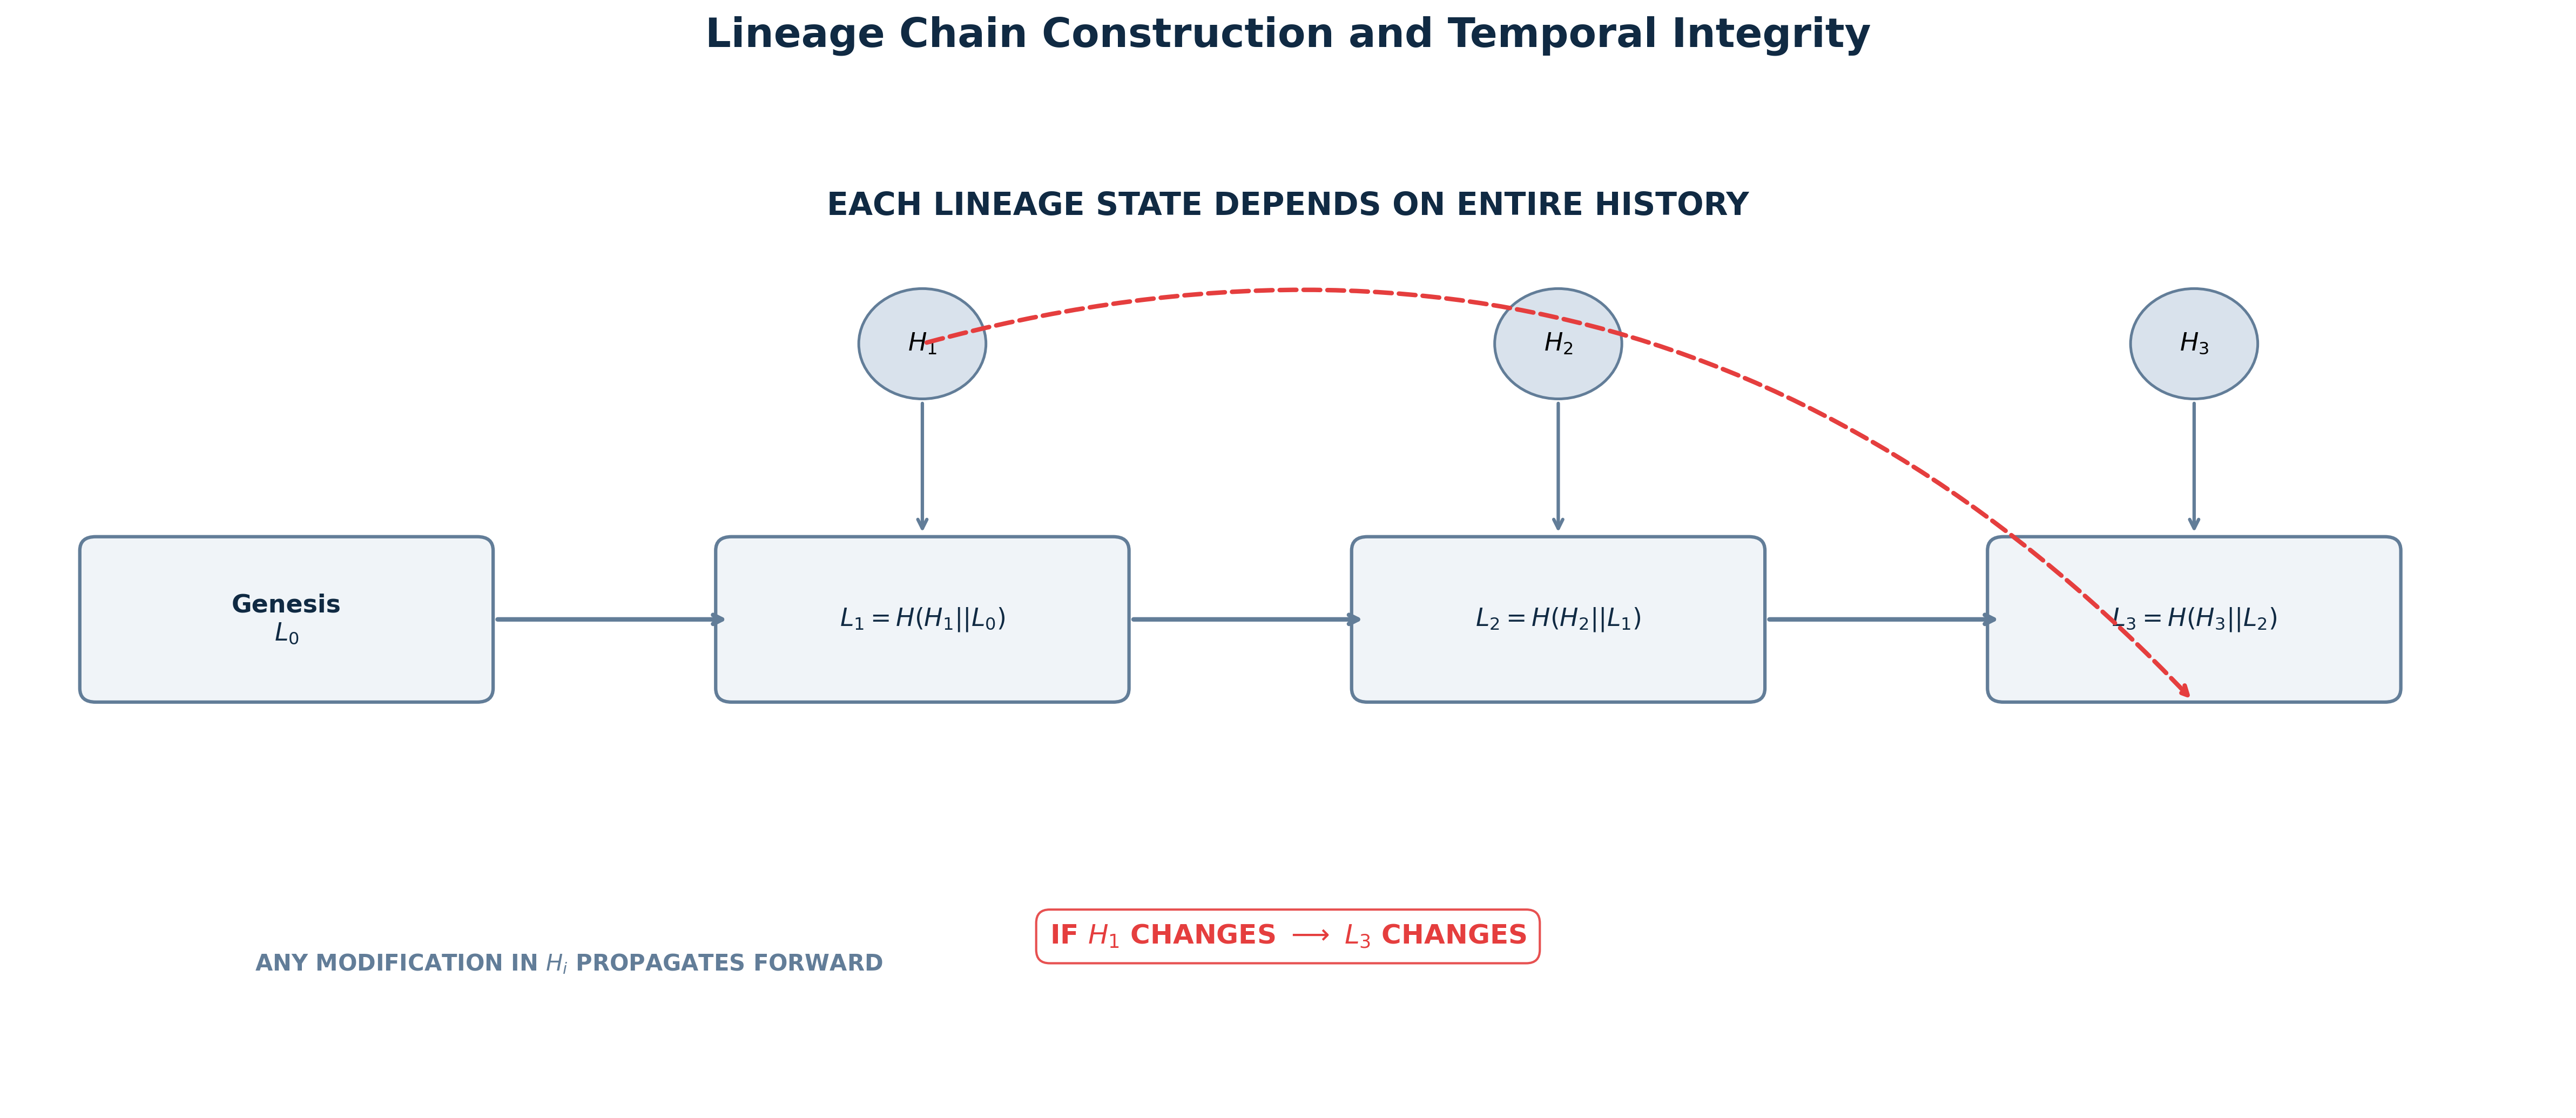
\includegraphics[width=\textwidth]{figures/2-Dimentionals/lineage_structure.png}
\caption{Cryptographic lineage chain construction linking telemetry batches via hash dependencies, ensuring forward integrity and tamper propagation.}
\label{fig:lineage}
\end{figure}

This recursive definition induces a chain structure in which each lineage value $L_t$ depends on all preceding telemetry elements.

\subsection{Lineage as a Cryptographic State Machine}

The lineage sequence may be interpreted as the evolution of a cryptographic state machine over the state space $\mathcal{L} = \{0,1\}^k$. The transition function is defined as:

\begin{equation}
L_t = \mathcal{F}_L(L_{t-1}, D_t) = \mathcal{H}(\mathcal{H}(\mathcal{S}(D_t)) \concat L_{t-1})
\end{equation}

This formulation reveals that the lineage state encapsulates the entire history of telemetry through iterative compression.

Let $\mathcal{L}_t$ denote the set of all possible lineage states at time $t$. Then:

\begin{equation}
|\mathcal{L}_t| \leq 2^k
\end{equation}

while the number of possible telemetry histories grows exponentially with $t$. The cryptographic properties of $\mathcal{H}$ ensure that distinct histories map to distinct lineage states with overwhelming probability.

\subsection{Forward Integrity Property}

A fundamental property of the lineage construction is forward integrity, which ensures that any modification to historical data propagates to all future lineage states.

\begin{theorem}[Forward Integrity]
Let $\{D_t\}$ and $\{D_t'\}$ be two telemetry sequences such that $D_k' \neq D_k$ for some $k < t$. Then:

\[
\Pr[L_t = L_t'] \leq 2^{-k}
\]
\end{theorem}

\begin{proof}
Assume $D_k' \neq D_k$. Then:

\[
H_k' = \mathcal{H}(\mathcal{S}(D_k')) \neq \mathcal{H}(\mathcal{S}(D_k)) = H_k
\]

with overwhelming probability due to collision resistance. Therefore:

\[
L_k' = \mathcal{H}(H_k' \concat L_{k-1}) \neq \mathcal{H}(H_k \concat L_{k-1}) = L_k
\]

Again, with overwhelming probability. By induction:

\[
L_{k+1}' = \mathcal{H}(H_{k+1} \concat L_k') \neq \mathcal{H}(H_{k+1} \concat L_k) = L_{k+1}
\]

and this inequality propagates forward to $L_t$. The only way for $L_t = L_t'$ is if a collision occurs in $\mathcal{H}$, which has probability at most $2^{-k}$.
\end{proof}

\subsection{Tamper Propagation and Detection}

The forward integrity property implies that any tampering with historical telemetry results in a mismatch in the current lineage state. Let $\Delta_t^L$ denote the lineage divergence:

\begin{equation}
\Delta_t^L = \| L_t - L_t' \|
\end{equation}

Then:

\begin{equation}
\Delta_t^L \neq 0 \quad \text{if any } D_k' \neq D_k \text{ for } k < t
\end{equation}

with overwhelming probability. This provides a mechanism for detecting tampering by comparing lineage values.

\subsection{Resistance to Truncation Attacks}

An adversary may attempt to truncate the telemetry sequence by removing entries beyond a certain index $k$. Let the original sequence be $\{D_0, \dots, D_t\}$ and the truncated sequence be $\{D_0, \dots, D_k\}$. The corresponding lineage states are $L_t$ and $L_k$.

The adversary may attempt to construct a new sequence $\{D_{k+1}', \dots, D_t'\}$ such that:

\begin{equation}
L_t' = L_t
\end{equation}

This requires finding inputs such that:

\begin{equation}
\mathcal{H}(H_t' \concat \dots \mathcal{H}(H_{k+1}' \concat L_k)) = L_t
\end{equation}

This is equivalent to a preimage attack on $\mathcal{H}$, which is computationally infeasible. Therefore, truncation attacks are prevented.

\subsection{Resistance to Reordering Attacks}

Consider a permutation $\pi$ applied to the telemetry sequence such that:

\begin{equation}
D_t' = D_{\pi(t)}
\end{equation}

Unless $\pi$ is the identity permutation, the sequence of content hashes $\{H_t'\}$ differs from $\{H_t\}$. Due to the recursive structure of the lineage, this results in:

\begin{equation}
L_t' \neq L_t
\end{equation}

with overwhelming probability. Thus, the lineage construction enforces strict ordering.

\subsection{Uniqueness of Lineage Representation}

The lineage function defines a mapping:

\begin{equation}
\mathcal{L}: \mathcal{D}^{t} \rightarrow \{0,1\}^k
\end{equation}

which is injective with high probability. That is:

\begin{equation}
\Pr[\mathcal{L}(D) = \mathcal{L}(D')] \leq 2^{-k} \quad \text{for } D \neq D'
\end{equation}

This ensures that the lineage uniquely identifies the telemetry history.

\subsection{Relation to Merkle Structures}

The lineage construction may be viewed as a degenerate Merkle tree in which each node has a single parent. Unlike traditional Merkle trees, which provide logarithmic verification paths for static datasets, the lineage construction provides constant-time verification for dynamic sequences.

Let $\mathcal{T}$ denote a Merkle tree and $\mathcal{L}$ the lineage. Then:

\begin{equation}
\mathcal{L}(D_0, \dots, D_t) = \mathcal{T}_{\text{linear}}(D_0, \dots, D_t)
\end{equation}

where $\mathcal{T}_{\text{linear}}$ is a tree with depth $t$ and branching factor $1$.

\subsection{Composability of Lineage}

The lineage construction is composable across segments. Let $\{D_0, \dots, D_k\}$ and $\{D_{k+1}, \dots, D_t\}$ be two segments. Then:

\begin{equation}
L_t = \mathcal{C}(L_k, \{D_{k+1}, \dots, D_t\})
\end{equation}

This property enables distributed processing and later recombination of telemetry segments.

\subsection{Entropy Accumulation}

Although each lineage state has fixed size $k$, it encodes information about the entire history. Let $H(D_0, \dots, D_t)$ denote the entropy of the telemetry sequence. Then:

\begin{equation}
H(L_t) \leq k
\end{equation}

but collision resistance ensures that distinct histories remain distinguishable.

\subsection{Implications for System Integrity}

The lineage construction enforces a global invariant:

\begin{equation}
L_t = \mathcal{H}(H_t \concat L_{t-1}) \quad \forall t
\end{equation}

which ensures that the telemetry sequence is immutable, ordered, and verifiable. Any deviation from this invariant results in a detectable inconsistency.

In summary, the Merkle-Lineage construction provides a cryptographic mechanism for enforcing temporal integrity over telemetry sequences. By embedding each element within a recursively defined hash chain, the protocol ensures that any modification, omission, or reordering of telemetry data is detectable with overwhelming probability. This construction forms the core of the RCO protocol's ability to guarantee tamper-evident and reproducible system behavior.

\section{Proof of Reflexion (PoR)}

While deterministic serialization and Merkle-lineage construction ensure structural integrity and temporal consistency of telemetry data, they do not, by themselves, guarantee that the telemetry originates from a legitimate computational process or that it accurately reflects the internal state of the system. The Proof of Reflexion (PoR) addresses this limitation by introducing a cryptographic mechanism that binds telemetry lineage to the originating computational state, thereby enforcing semantic integrity in addition to structural integrity.

\begin{figure}[htbp]
\centering
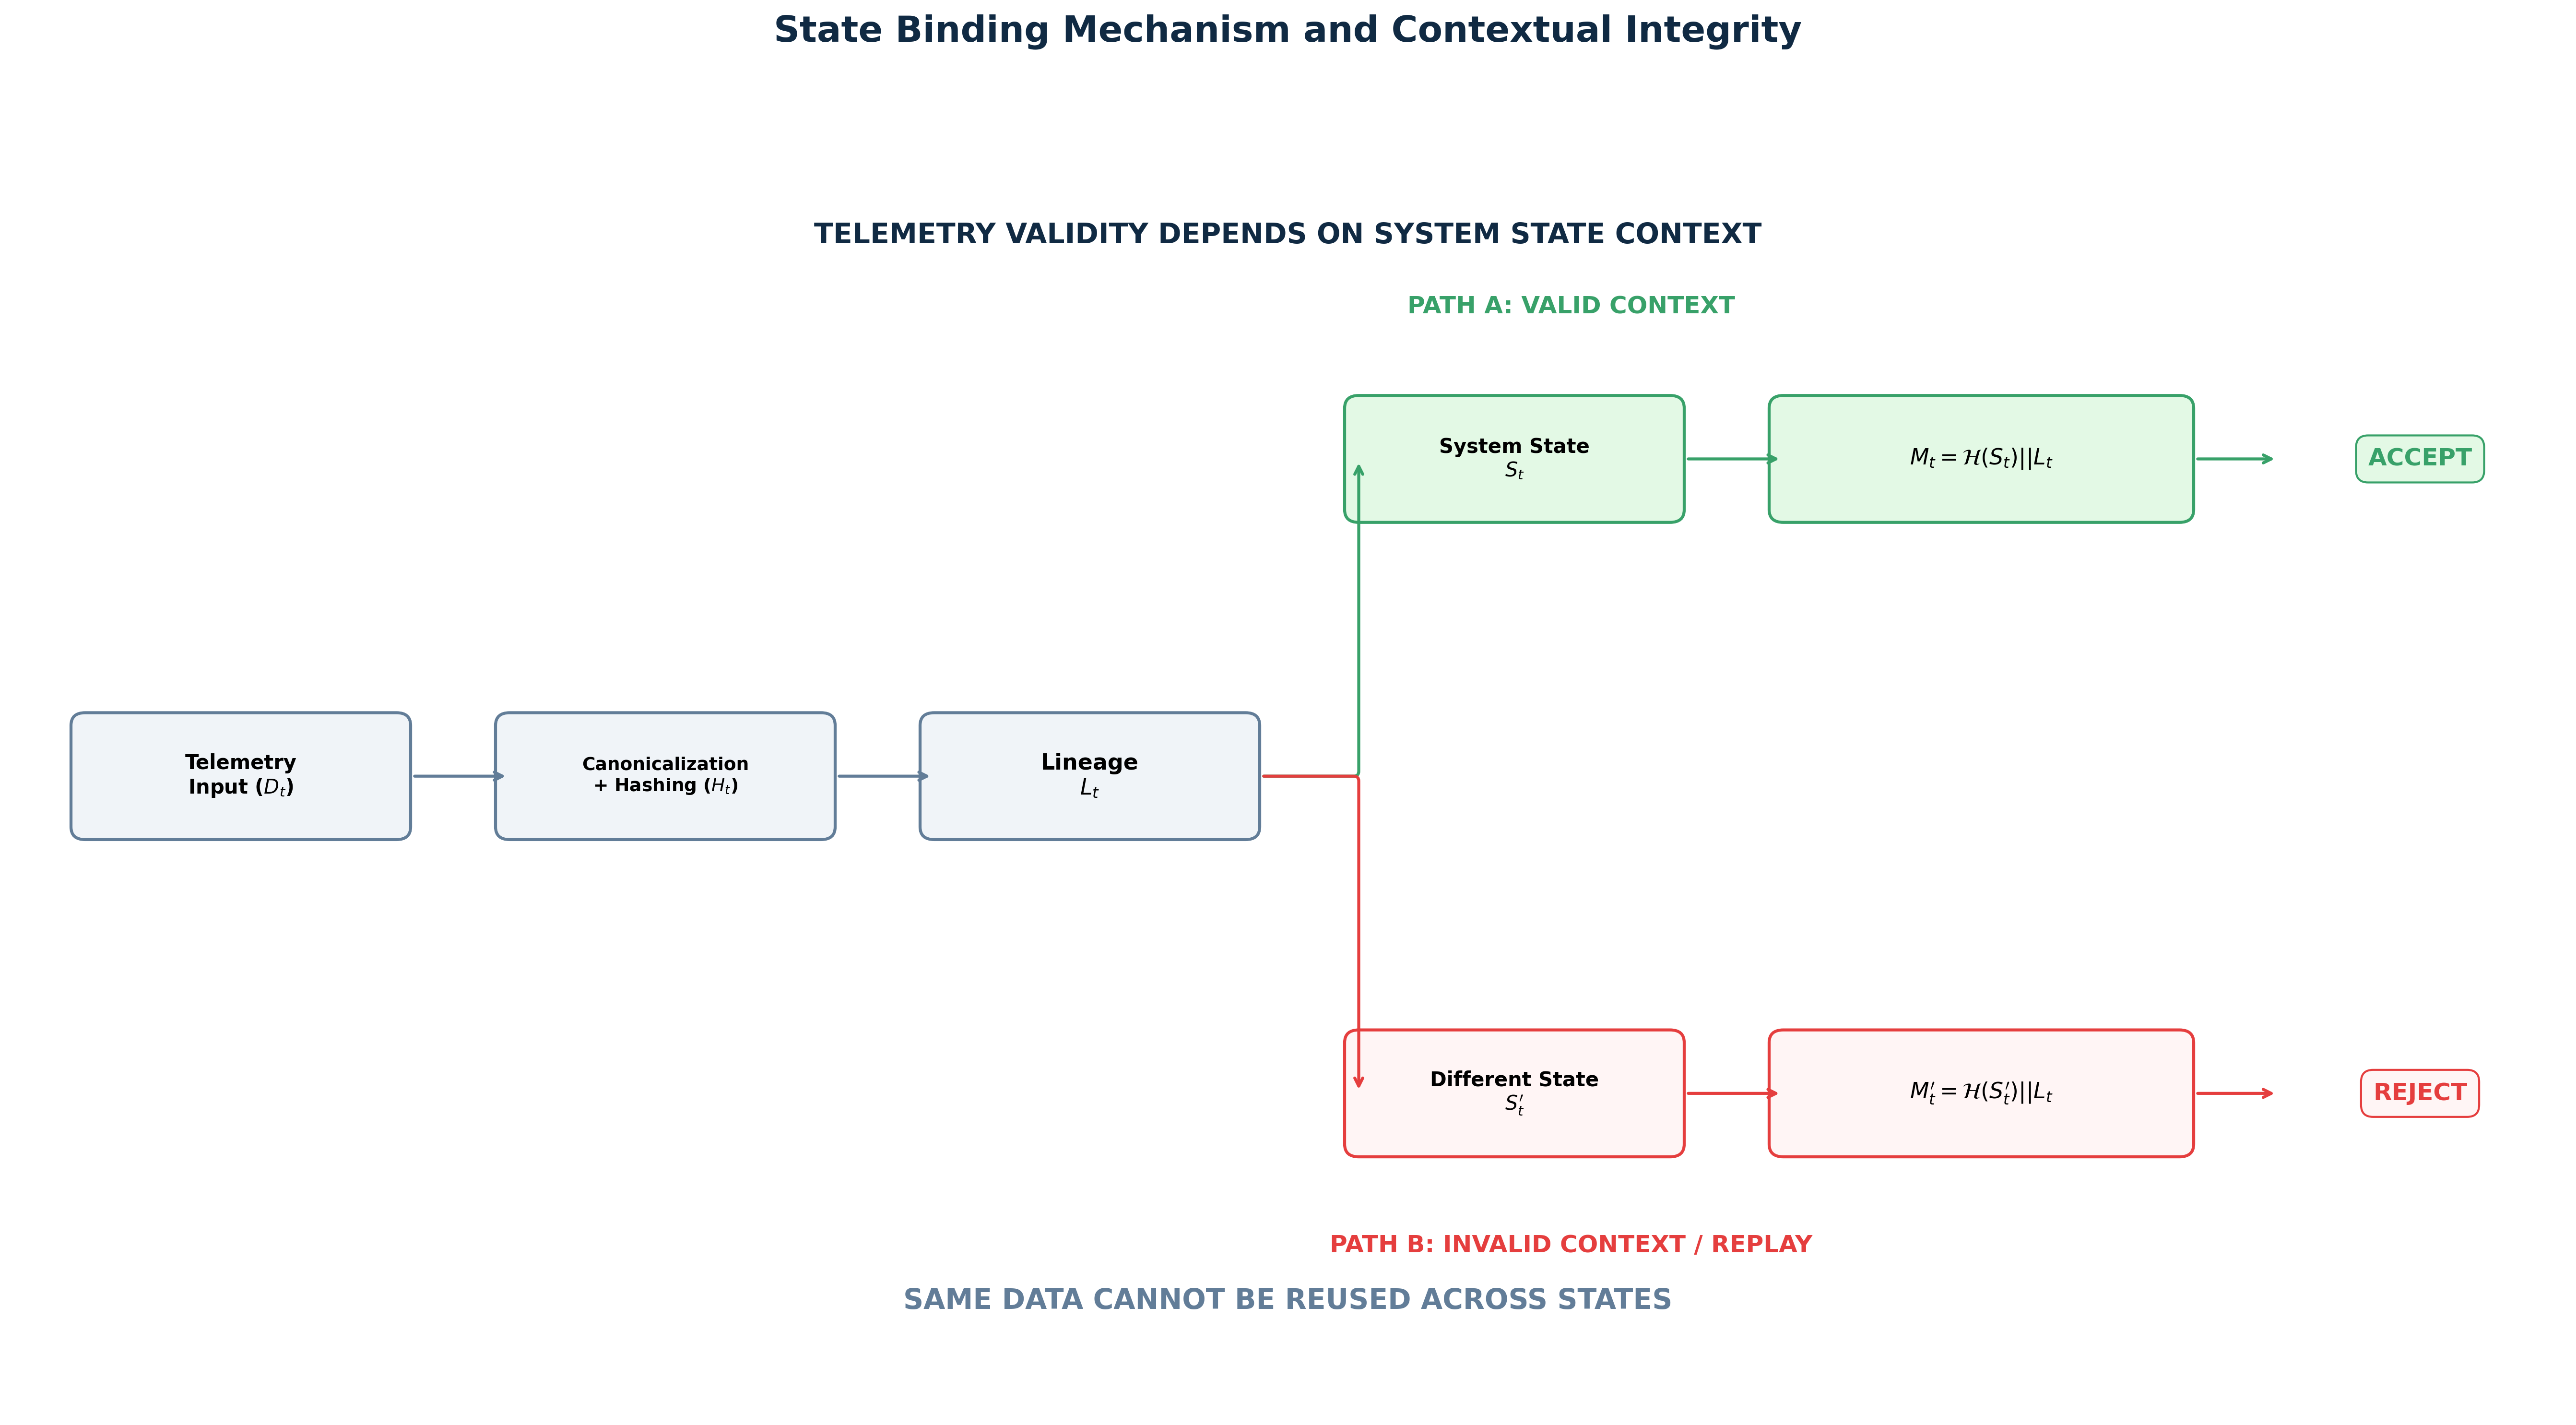
\includegraphics[width=\textwidth]{figures/2-Dimentionals/state_binding.png}
\caption{State binding mechanism associating telemetry with originating computational state, forming the basis of Proof of Reflexion.}
\label{fig:state-binding}
\end{figure}

The central concept underlying PoR is that telemetry disclosures must not only be consistent and immutable but must also be reflexively derived from the internal state of the system. This requirement is formalized by establishing a cryptographic dependency between the lineage state $L_t$ and a representation of the system state $S_t$.

\subsection{Formal Definition of Reflexive Binding}

Let $\mathcal{H}_S: \mathcal{S} \rightarrow \{0,1\}^k$ denote a state hashing function that maps the system state to a fixed-length digest. The reflexive binding condition requires that for each telemetry element $D_t$:

\begin{equation}
D_t = \mathcal{G}(S_t)
\end{equation}

for some observation function $\mathcal{G}$. The Proof of Reflexion enforces this relationship indirectly by constructing a cryptographic proof:

\begin{equation}
\Sigma_t = \text{Sign}(\mathcal{H}_S(S_t) \concat L_t, K)
\end{equation}

where $K$ is a private key associated with the computational entity.

This construction ensures that the proof $\Sigma_t$ is a function of both the lineage and the internal state, thereby binding the two.

\subsection{Verification Condition}

Given a public key $PK$, the verification operator evaluates:

\begin{equation}
\mathcal{V}_{\text{PoR}}(S_t, L_t, \Sigma_t) = \text{Verify}(\mathcal{H}_S(S_t) \concat L_t, \Sigma_t, PK)
\end{equation}

The proof is considered valid if and only if:

\begin{equation}
\mathcal{V}_{\text{PoR}}(S_t, L_t, \Sigma_t) = \text{true}
\end{equation}

This condition ensures that the lineage $L_t$ is cryptographically bound to a valid state representation.

\subsection{State Consistency Guarantee}

The PoR mechanism enforces that any valid telemetry entry must correspond to a state $S_t$ satisfying:

\begin{equation}
\Sigma_t = \text{Sign}(\mathcal{H}_S(S_t) \concat L_t, K)
\end{equation}

An adversary attempting to produce a valid proof for a falsified telemetry element $D_t'$ must either:

\begin{equation}
\text{(i)} \quad \mathcal{H}_S(S_t') = \mathcal{H}_S(S_t)
\end{equation}

or:

\begin{equation}
\text{(ii)} \quad \text{forge } \Sigma_t
\end{equation}

The first condition corresponds to a collision in the state hash function, while the second corresponds to a signature forgery.

\subsection{Unforgeability Theorem}

\begin{theorem}[PoR Unforgeability]
Assuming that the signature scheme is existentially unforgeable under chosen-message attacks (EUF-CMA) and that $\mathcal{H}_S$ is collision-resistant, an adversary cannot produce a valid proof $\Sigma_t'$ for a falsified pair $(S_t', L_t)$ without access to the private key $K$.
\end{theorem}

\begin{proof}
Suppose an adversary $\mathcal{A}$ produces a valid proof $\Sigma_t'$ for $(S_t', L_t)$ such that:

\[
\text{Verify}(\mathcal{H}_S(S_t') \concat L_t, \Sigma_t', PK) = \text{true}
\]

There are two possibilities:

1. $\mathcal{H}_S(S_t') = \mathcal{H}_S(S_t)$, implying a collision in $\mathcal{H}_S$.

2. $\Sigma_t'$ is a valid signature on a new message $\mathcal{H}_S(S_t') \concat L_t$.

The first case contradicts the collision resistance of $\mathcal{H}_S$. The second case contradicts the EUF-CMA security of the signature scheme. Therefore, the adversary cannot succeed except with negligible probability.
\end{proof}

\subsection{Resistance to State Substitution Attacks}

An adversary may attempt to substitute the system state while preserving the lineage. Let $(S_t, L_t)$ be a valid pair and $(S_t', L_t)$ a substituted pair. The adversary must produce:

\begin{equation}
\Sigma_t' = \text{Sign}(\mathcal{H}_S(S_t') \concat L_t, K)
\end{equation}

Without access to $K$, this is infeasible. Thus, the PoR mechanism prevents substitution of system state without detection.

\subsection{Binding Strength Analysis}

The strength of the binding between $S_t$ and $L_t$ depends on the entropy of $\mathcal{H}_S(S_t)$. Let:

\begin{equation}
H(\mathcal{H}_S(S_t)) = k
\end{equation}

Then the probability of a collision is bounded by:

\begin{equation}
\Pr[\mathcal{H}_S(S_t) = \mathcal{H}_S(S_t')] \leq 2^{-k}
\end{equation}

This ensures that the binding is strong and resistant to collision-based attacks.

\subsection{Extension to Threshold Proofs}

In a distributed setting, the PoR mechanism may be extended to a threshold signature scheme. Let $K_i$ denote key shares held by validators. Each validator produces:

\begin{equation}
\sigma_i = \text{Sign}(\mathcal{H}_S(S_t) \concat L_t, K_i)
\end{equation}

An aggregate proof is constructed as:

\begin{equation}
\Sigma_t = \text{Aggregate}(\sigma_{i_1}, \dots, \sigma_{i_m})
\end{equation}

for $m \geq t$, where $t$ is the threshold. The verification condition remains:

\begin{equation}
\text{Verify}(\mathcal{H}_S(S_t) \concat L_t, \Sigma_t, PK) = \text{true}
\end{equation}

This extension provides resilience against Byzantine faults.

\subsection{Separation from Classical Signatures}

It is important to distinguish PoR from classical digital signatures. In standard systems, signatures are applied directly to data:

\begin{equation}
\Sigma_t = \text{Sign}(D_t, K)
\end{equation}

This provides authenticity but does not guarantee that $D_t$ is consistent with the system state. In contrast, PoR signs a composite message:

\begin{equation}
\mathcal{H}_S(S_t) \concat L_t
\end{equation}

which encodes both the lineage and the state, thereby enforcing a stronger integrity condition.

\subsection{Reflexive Integrity Condition}

The PoR mechanism enforces the following invariant:

\begin{equation}
\text{Valid}(D_t) \implies \exists S_t \text{ such that } D_t = \mathcal{G}(S_t) \land \text{Verify}(\mathcal{H}_S(S_t) \concat L_t, \Sigma_t)
\end{equation}

This condition ensures that valid telemetry is both structurally correct and semantically consistent.

\subsection{Implications for System Security}

By binding telemetry lineage to system state, the PoR mechanism eliminates a critical class of attacks in which adversaries generate structurally valid but semantically incorrect telemetry. Combined with the lineage construction, this ensures that telemetry data is both tamper-evident and state-consistent.

In summary, the Proof of Reflexion introduces a novel cryptographic mechanism that extends traditional integrity guarantees to include state provenance. By binding telemetry to the originating computational state, the RCO protocol ensures that data is not only consistent and immutable but also semantically valid, thereby addressing a fundamental limitation of existing systems.

\section{Unified Integrity Model and Security Composition}

The preceding sections have introduced the individual components of the cryptographic core, namely deterministic serialization, cryptographic hashing, Merkle-lineage construction, and Proof of Reflexion. Each component enforces a specific invariant necessary for ensuring the integrity of telemetry data in feedback-coupled computational systems. However, the full strength of the RCO protocol emerges only when these components are composed into a unified framework that enforces a global integrity condition.

Let the telemetry processing pipeline be defined as the composition:

\begin{equation}
\mathcal{P}_{\text{RCO}} = \mathcal{V}_{\text{PoR}} \circ \mathcal{S}_{\text{PoR}} \circ \mathcal{C} \circ \mathcal{H} \circ \mathcal{S}
\end{equation}

where $\mathcal{S}$ is the canonical serialization operator, $\mathcal{H}$ is the cryptographic hashing operator, $\mathcal{C}$ is the lineage construction operator, $\mathcal{S}_{\text{PoR}}$ is the proof generation operator, and $\mathcal{V}_{\text{PoR}}$ is the verification operator.

The pipeline $\mathcal{P}_{\text{RCO}}$ defines a mapping:

\begin{equation}
\mathcal{P}_{\text{RCO}}: \mathcal{D} \times \mathcal{S} \rightarrow \{\text{true}, \text{false}\}
\end{equation}

which determines whether a telemetry element is valid.

\subsection{Composite Validity Condition}

A telemetry element $D_t$ is considered valid if and only if the following composite condition is satisfied:

\begin{equation}
\text{Valid}(D_t) \iff
\begin{cases}
\mathcal{S}(D_t) \text{ is canonical} \\
H_t = \mathcal{H}(\mathcal{S}(D_t)) \\
L_t = \mathcal{H}(H_t \concat L_{t-1}) \\
\Sigma_t = \text{Sign}(\mathcal{H}_S(S_t) \concat L_t, K) \\
\text{Verify}(\mathcal{H}_S(S_t) \concat L_t, \Sigma_t, PK) = \text{true}
\end{cases}
\end{equation}

This condition integrates representation determinism, structural integrity, temporal continuity, and state provenance into a single verification criterion.

\subsection{Global Integrity Theorem}

\begin{theorem}[Global Integrity of RCO]
Assuming that the serialization function $\mathcal{S}$ is canonical, the hash function $\mathcal{H}$ is collision-resistant, the state hash function $\mathcal{H}_S$ is collision-resistant, and the signature scheme is EUF-CMA secure, the RCO pipeline satisfies the following property:

\[
\forall D, \tilde{D}, \quad \mathcal{P}_{\text{RCO}}(D) = \mathcal{P}_{\text{RCO}}(\tilde{D}) = \text{true} \implies D \equiv \tilde{D}
\]

with overwhelming probability.
\end{theorem}

\begin{proof}
Assume $\mathcal{P}_{\text{RCO}}(D) = \mathcal{P}_{\text{RCO}}(\tilde{D}) = \text{true}$. Then both inputs satisfy the composite validity condition.

From canonical serialization:

\[
\mathcal{S}(D) = \mathcal{S}(\tilde{D}) \implies D \equiv \tilde{D}
\]

Otherwise, if $D \not\equiv \tilde{D}$, then:

\[
\mathcal{S}(D) \neq \mathcal{S}(\tilde{D})
\]

which implies:

\[
\mathcal{H}(\mathcal{S}(D)) \neq \mathcal{H}(\mathcal{S}(\tilde{D}))
\]

with overwhelming probability due to collision resistance. This leads to:

\[
H_t \neq \tilde{H}_t \implies L_t \neq \tilde{L}_t
\]

by the forward integrity of the lineage construction.

Finally, any attempt to produce valid proofs $\Sigma_t$ and $\tilde{\Sigma}_t$ for inconsistent lineage states or system states would require either forging a signature or finding a collision in $\mathcal{H}_S$, both of which are infeasible under the given assumptions.

Therefore, $D \equiv \tilde{D}$ must hold, completing the proof.
\end{proof}

\subsection{Elimination of the Perturbation Channel}

From the system dynamics established in Chapter 01, telemetry-induced perturbations are represented by $\delta_t$. Under the RCO protocol, the validity condition enforces:

\begin{equation}
\delta_t = 0 \quad \forall t
\end{equation}

with respect to representation and structural integrity. Substituting into the divergence relation:

\begin{equation}
\Delta_{t+1} \leq L_s \Delta_t + L_d \|\delta_t\|
\end{equation}

yields:

\begin{equation}
\Delta_{t+1} \leq L_s \Delta_t
\end{equation}

which ensures that system evolution is deterministic and free from telemetry-induced distortion.

\subsection{Security Reduction}

The security of the RCO protocol may be reduced to the security of its underlying primitives. Let $\mathcal{A}$ be an adversary attempting to violate the integrity of the system. Then $\mathcal{A}$ must succeed in at least one of the following:

\begin{equation}
\text{(i)} \quad \text{Break canonical determinism of } \mathcal{S}
\end{equation}

\begin{equation}
\text{(ii)} \quad \text{Find a collision in } \mathcal{H}
\end{equation}

\begin{equation}
\text{(iii)} \quad \text{Find a collision in } \mathcal{H}_S
\end{equation}

\begin{equation}
\text{(iv)} \quad \text{Forge a signature under EUF-CMA}
\end{equation}

Thus, the overall security is bounded by:

\begin{equation}
\Pr[\text{Break RCO}] \leq \epsilon_{\mathcal{S}} + \epsilon_{\mathcal{H}} + \epsilon_{\mathcal{H}_S} + \epsilon_{\text{sig}}
\end{equation}

where each term is negligible.

\subsection{Minimal Integrity Composition}

In the Minimal Viable Integrity Model, the pipeline reduces to:

\begin{equation}
\mathcal{P}_{\text{MVI}} = \mathcal{C} \circ \mathcal{H} \circ \mathcal{S}
\end{equation}

The corresponding validity condition is:

\begin{equation}
\text{Valid}_{\text{MVI}}(D_t) \iff L_t = \mathcal{H}(\mathcal{H}(\mathcal{S}(D_t)) \concat L_{t-1})
\end{equation}

This ensures structural and temporal integrity but does not enforce state provenance.

\subsection{Compositional Closure}

The RCO pipeline is closed under composition in the sense that multiple pipelines may be combined while preserving integrity. Let $\mathcal{P}_1$ and $\mathcal{P}_2$ be two valid pipelines. Then:

\begin{equation}
\mathcal{P}_{\text{combined}} = \mathcal{P}_2 \circ \mathcal{P}_1
\end{equation}

satisfies the same integrity condition, provided that the output of $\mathcal{P}_1$ conforms to the input requirements of $\mathcal{P}_2$.

\subsection{Final Integrity Invariant}

The RCO protocol enforces the following global invariant over the telemetry sequence:

\begin{equation}
\forall t, \quad \text{Valid}(D_t) = \text{true} \implies
\begin{cases}
D_t \text{ is deterministically represented} \\
\text{The sequence } \{D_0, \dots, D_t\} \text{ is immutable} \\
D_t \text{ is consistent with } S_t \\
\text{The lineage } L_t \text{ uniquely identifies the history}
\end{cases}
\end{equation}

This invariant encapsulates the complete integrity guarantees of the protocol.

\subsection{Conclusion}

The unified cryptographic core of the RCO protocol establishes a formally verified framework for ensuring the integrity of telemetry data in feedback-coupled systems. By composing deterministic serialization, cryptographic hashing, lineage construction, and Proof of Reflexion, the protocol enforces a comprehensive set of invariants that eliminate ambiguity, prevent tampering, and ensure consistency between telemetry and system state.

This unified model not only addresses the deficiencies of existing systems but also provides a foundation for the development of high-assurance computational infrastructures in which telemetry integrity is treated as a first-class requirement.